\subsubsection{Attitude Controller Simulation}\label{sec:AttSim}
The design for the state feedback and the observer are provided. The final attitude response, step response and observer estimation can are analyzed and discussed. The controller and observer gains are changed in the different simulations to illustrate why the final design is chosen.

%A short description for the following three simulations in \autoref{fig:ssFinalEq}, \autoref{fig:ssObsFinal} and \autoref{fig:ssFinalStep} is given. For the final attitude controller, the weighted matrices, $\vec{Q_{final}}$ and $\vec{R_{final}}$, and the observer gain, $\vec{L_{obs}}$. These can be found in \autoref{app:matricesSS}.

In \autoref{fig:ssFinalEq}, the simulated angle response of the final attitude controller is shown. Initial conditions are given to the three angles. These are set to $0.2$ rad for the pitch, $-0.3$ for the roll and $-0.2$ for the yaw. This shows how the controller stabilizes the attitude around 0 rad.
%
\begin{figure}[H]
	\centering
	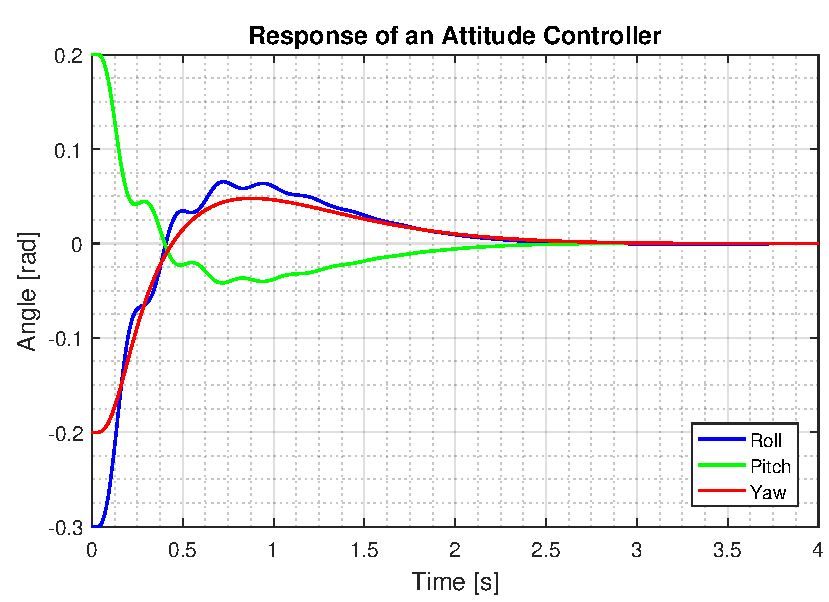
\includegraphics[scale=0.8]{figures/ssFinalEq.pdf}
	\caption{System response of the attitude controller, with initial conditions of $0.2$ radians for the pitch, $-0.3$ radians for the roll and $-0.2$ radians for the yaw. The weighted matrices, $\vec{Q_{final}}$ and $\vec{R_{final}}$, and the observer gain, $\vec{L_{obs}}$, are utilized for the final design and can be found in \autoref{app:matricesSS}.}
	\label{fig:ssFinalEq}
\end{figure}
%

It can be seen from the figure that it approximately takes $2.5$ \si{s} for the pitch and roll to settle at zero, where it only takes approximately $1.4$-$1.5$ \si{s} for the yaw.

In \autoref{fig:ssObsFinal}, the estimation for the angular velocities, done with the same conditions as in \autoref{fig:ssFinalEq}, is depicted. To be able to evaluate the observers estimation (red line), it is compared with the actual angular velocity (blue line). \\  
%
\begin{figure}[H]
	\centering
	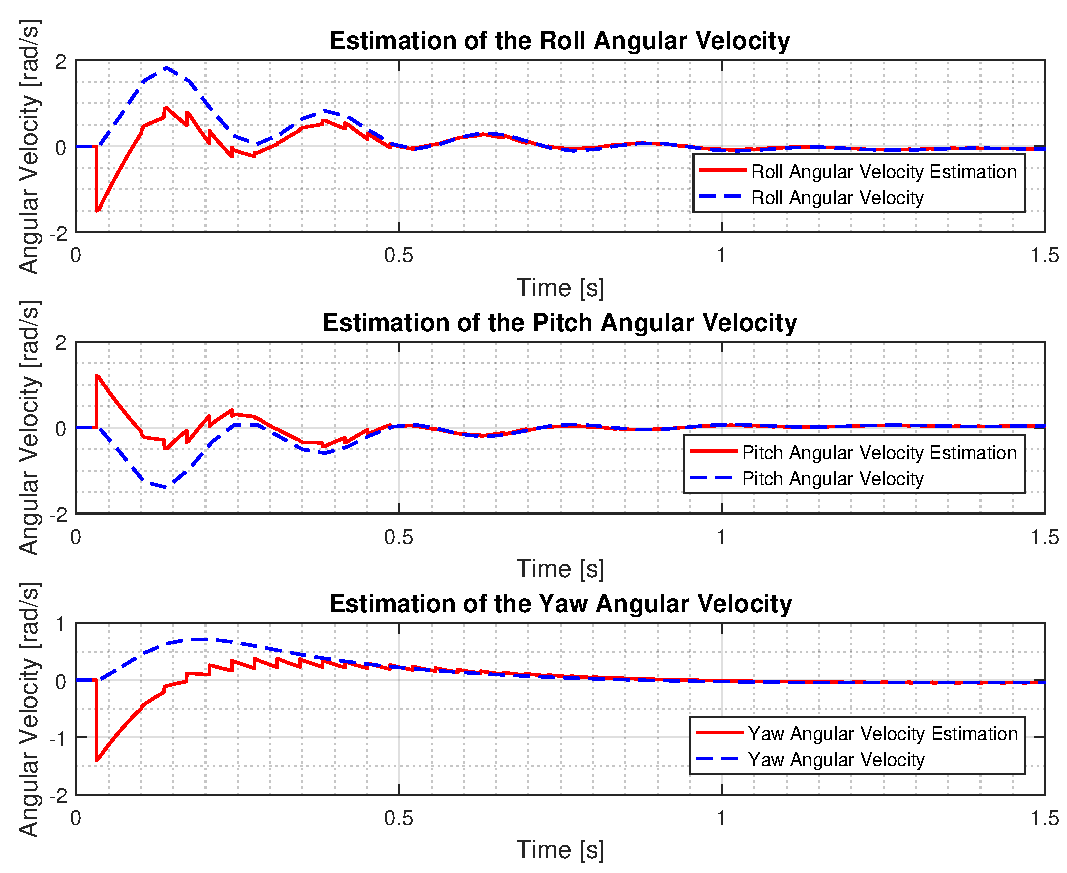
\includegraphics[scale=0.7]{figures/ssObsFinal.pdf}
	\caption{The three figures shows the estimation of the angular velocities made by the implemented observer. The simulations initial conditions for roll, pitch and yaw are identical to the simulation in \autoref{fig:ssFinalEq}. The utilized weighted matrices, $\vec{Q_{final}}$ and $\vec{R_{final}}$, and the observer gain, $\vec{L_{obs}}$, can be found in \autoref{app:matricesSS}.}
	\label{fig:ssObsFinal}
\end{figure}
%
The estimations' large spikes in the beginning of the figures are due to the initial conditions for the angles. The large gap between the actual and the estimation, is due to multiple factors. The main issue is the convergence of the estimate to the real value as the dynamics of the observer do not allow a instantaneous estimation. Also, the delay and sampling frequency affects the estimation creating the spikes seen in the plot. %Furthermore the observer utilizes the created model for the quadcopter, see \autoref{chap:Model}. As the model is not a perfect replica of how the system behaves in reality, errors are unavoidable. The small triangular spikes are both due to the sampling rate and the integrator in the observer. Each time the observer receives new angles the steep increase or decrease occur. As there is an integrator in the observer the estimation either decreases or increases until new angles is received $35$ \si{ms} later.

A step response of the roll is shown in \autoref{fig:ssFinalStep}. As the roll and the pitch are implemented identically, the step response of the two are similar. Additionally, the yaw is not illustrated as the reference is set to zero. It is therefore only desired to discover how the roll and pitch track a reference. 
%
\begin{figure}[H]
	\centering
	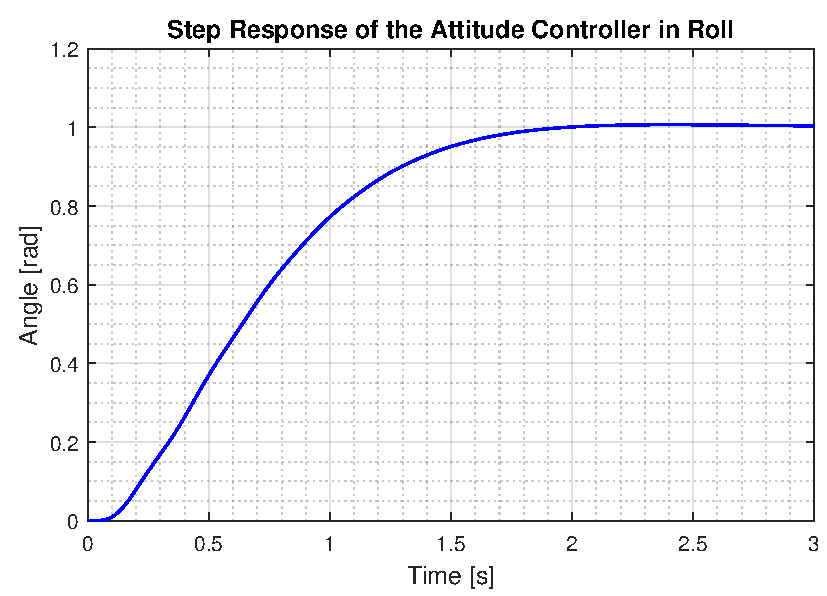
\includegraphics[scale=0.8]{figures/ssFinalStep.pdf}
	\caption{An step response of the final system. This illustrates only the behavior of the roll, as the yaw is always set to zero and the pitch would be identical to the roll. The utilized weighted matrices, $\vec{Q_{final}}$ and $\vec{R_{final}}$, and the observer gain, $\vec{L_{obs}}$, can be found in \autoref{app:matricesSS}.}
	\label{fig:ssFinalStep}
\end{figure}
%
The system is subjected to a step input reference of \SI{1}{m s^{-1}}. With an error band of 5 percent, the settling time is approximately $1.5$ \si{s} and the overshoot is less than 5 percent. \fxnote{write something about why 1.5 is okay?}

To illustrate the reasoning followed to find the final design, two more simulations are shown, where the controller and observer matrices are changed one at a time, so that it is possible to compare the different simulations with the final design and discuss why the final parameters are chosen.

The changed matrices, called $\vec{Q_{high}}$ and $\vec{R_{high}}$ can be seen in \autoref{app:matricesSS}. Compared to the final design the allowed state error in the angles is less and the allowed control action is increased. These changes should yield a more reactive system. This can be seen in the angle response shown in \autoref{fig:ssEqBad}. Note that the initial conditions for the response are the same as for \autoref{fig:ssFinalEq}.
%
\begin{figure}[H]
	\centering
	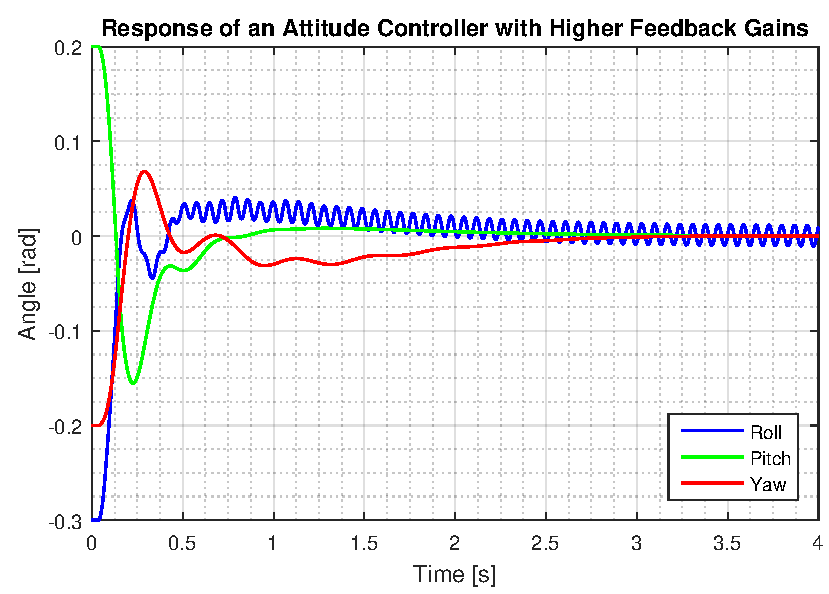
\includegraphics[scale=1]{figures/ssEqBad.pdf}
	\caption{Attitude controller response utilizing the weighted matrices, $\vec{Q_{high}}$ and $\vec{R_{high}}$, and the observer gain, $\vec{L_{obs}}$, found in \autoref{app:matricesSS}. The initial conditions for the angles is set to $0.2$ radians for the pitch, $-0.3$ radians for the roll and $-0.2$ radians for the yaw.}
	\label{fig:ssEqBad}
\end{figure}
%
It can be seen from \autoref{fig:ssEqBad} that the roll shows an oscillatory behavior. The network effects in the system and the more reactive controller cause this response.%is not able to stabilize the roll. Since the absolute value for the initial conditions for roll is larger than the pitch, it is the roll which is oscillating in this simulation. From this 
It is possible to conclude that a higher feedback gain compared to the final utilized gain is not desired for the attitude controller.

The observer gain, $\vec{L_{obsH}}$, utilized for the simulation in  \autoref{fig:TranslationalControlDiagram} is increased compared to the observer gain utilized in the final design. This results in more oscillations in both the pitch and the roll. Additionally, the yaw takes more time to settle compared to the actual value shown in \autoref{fig:ssFinalEq}. It is seen that when increasing the gain the observer is worse at estimating the angular velocity compared to the final design mainly due to the delay and sampling time effect.
%
\begin{figure}[H]
	\centering
	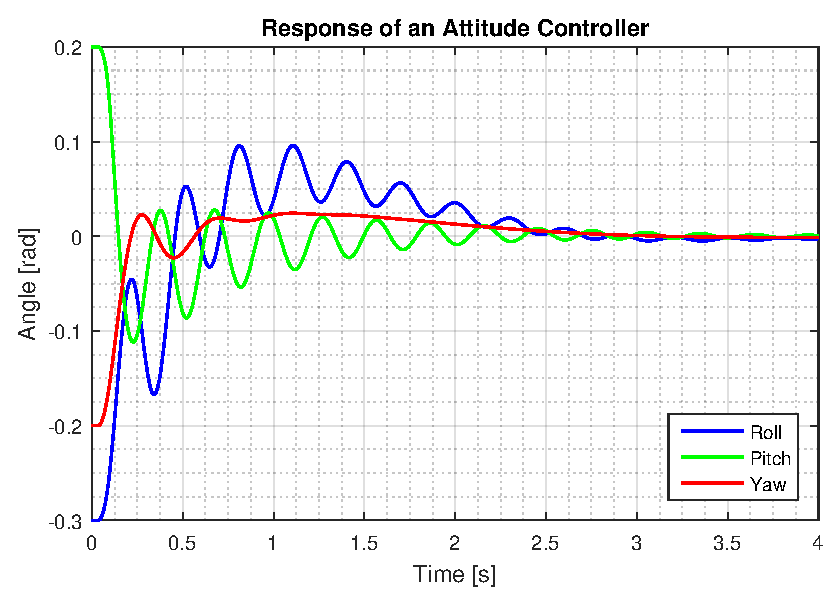
\includegraphics[scale=0.8]{figures/ssEqObsHigh.pdf}
	\caption{Angle response with an increase in the observer gain compared to the final design. The utilized weighted matrices, $\vec{Q_{final}}$ and $\vec{R_{final}}$, and the observer gain, $\vec{L_{obsH}}$ can be found in \autoref{app:matricesSS}.}
	\label{fig:TranslationalControlDiagram}
\end{figure}
%
From the simulations in \autoref{fig:TranslationalControlDiagram} and \autoref{fig:TranslationalControlDiagram} it is evident that an increase in gain in either the state feedback or in the observer is not desired compared to the final design.

The final attitude controller is therefore a compromise between a fast system, with oscillating behavior, and a slower system without oscillating behavior.


